Auf Grundlage der zuvor genannten Messvoraussetzungen konnte die Roboter-Gesten-Anwen-\\dung verschiedenen Tests unterzogen und deren Ergebnisse ausgewertet werden. Zur Durchführung der Tests wurde die Roboter-Gesten-Anwendung mit zusätzlichen \quoteMark{*\_MEASUREMENT}-Flags, zu denen die Flags \quoteMark{GESTURE\_MEASUREMENT}, \quoteMark{COMMUNICATION\_MEASU-\\REMENT} und \quoteMark{POSITION\_MEASUREMENT} zählen, kompiliert um ausführliche Statistikdaten für den jeweils durchgeführten Testfall zu erhalten. Die durchgeführten Tests reichen hierbei von Latenztests der Gestenerkennung mittels der Azure Kinect über Latenztests der Kommunikation mittels ROS und der direkten Kommunikation mit dem \quoteMark{WidowX 200}-Lernroboter bis hin zu der Genauigkeit der anzufahrenden Zielpositionen. Die erhobenen statistischen Daten wurden analysiert und werden nachfolgend mittels Diagrammen veranschaulicht und kritisch hinterfragt.

\section{Latenz der Gestenerkennung}
Zum Testen der Latenz der Gestenerkennung wurde das Azure Kinect Body Tracking SDK im CPU-Modus anstatt mit der Grafikkartenbeschleunigung gestartet. Dies war notwendig, da eine Grafikkarte von AMD statt einer Nvidia Grafikkarte im Testsystem eingesetzt wird. Zudem kann hiermit der kleinste gemeinsame Nenner der im Umlauf befindlicher Systeme widergespiegelt werden, welche keine propritären Features von Nvidia Grafikkarten, wie z.B. CUDA, verwenden. Die Latenz der Gestenerkennung beinhaltet die Zeit vom Aussenden des Infrarot-Lichtimpuls bis zum Empfang und Absorption des Lichtimpuls bis hin zur Latenz über das \quoteMark{USB 3.0}-Kabel und der Verarbeitung der Daten durch das Azure Kinect Body Tracking SDK. Zum Testen der Latenz der Gestenerkennung wurde die Roboter-Gesten-Anwendung und deren Abhängigkeiten mittels der Flags \quoteMark{MEASUREMENT} und \quoteMark{GESTURE\_MEASUREMENT}, welche im Anhang \ref{appendix1.2:Installation_und_Konfiguration_der_Pakete} aufgezeigt werden, kompiliert. Bei der Durchführung des Tests wurden von dem Proband die in dieser Arbeit entwickelten Gesten abwechselnd in zufälliger Reihenfolge vor der Azure Kinect ausgeführt. Die Datei \quoteMark{Messung der Gestenerkennung.csv}, welche bei der Durchführung des Tests von der Roboter-Gesten-Anwendung erstellt wurde, ist auf dem Beilagemedium im Verzeichnis \quoteMark{Testdaten/} zu finden.

\begin{figure}[htb]
	\centering
	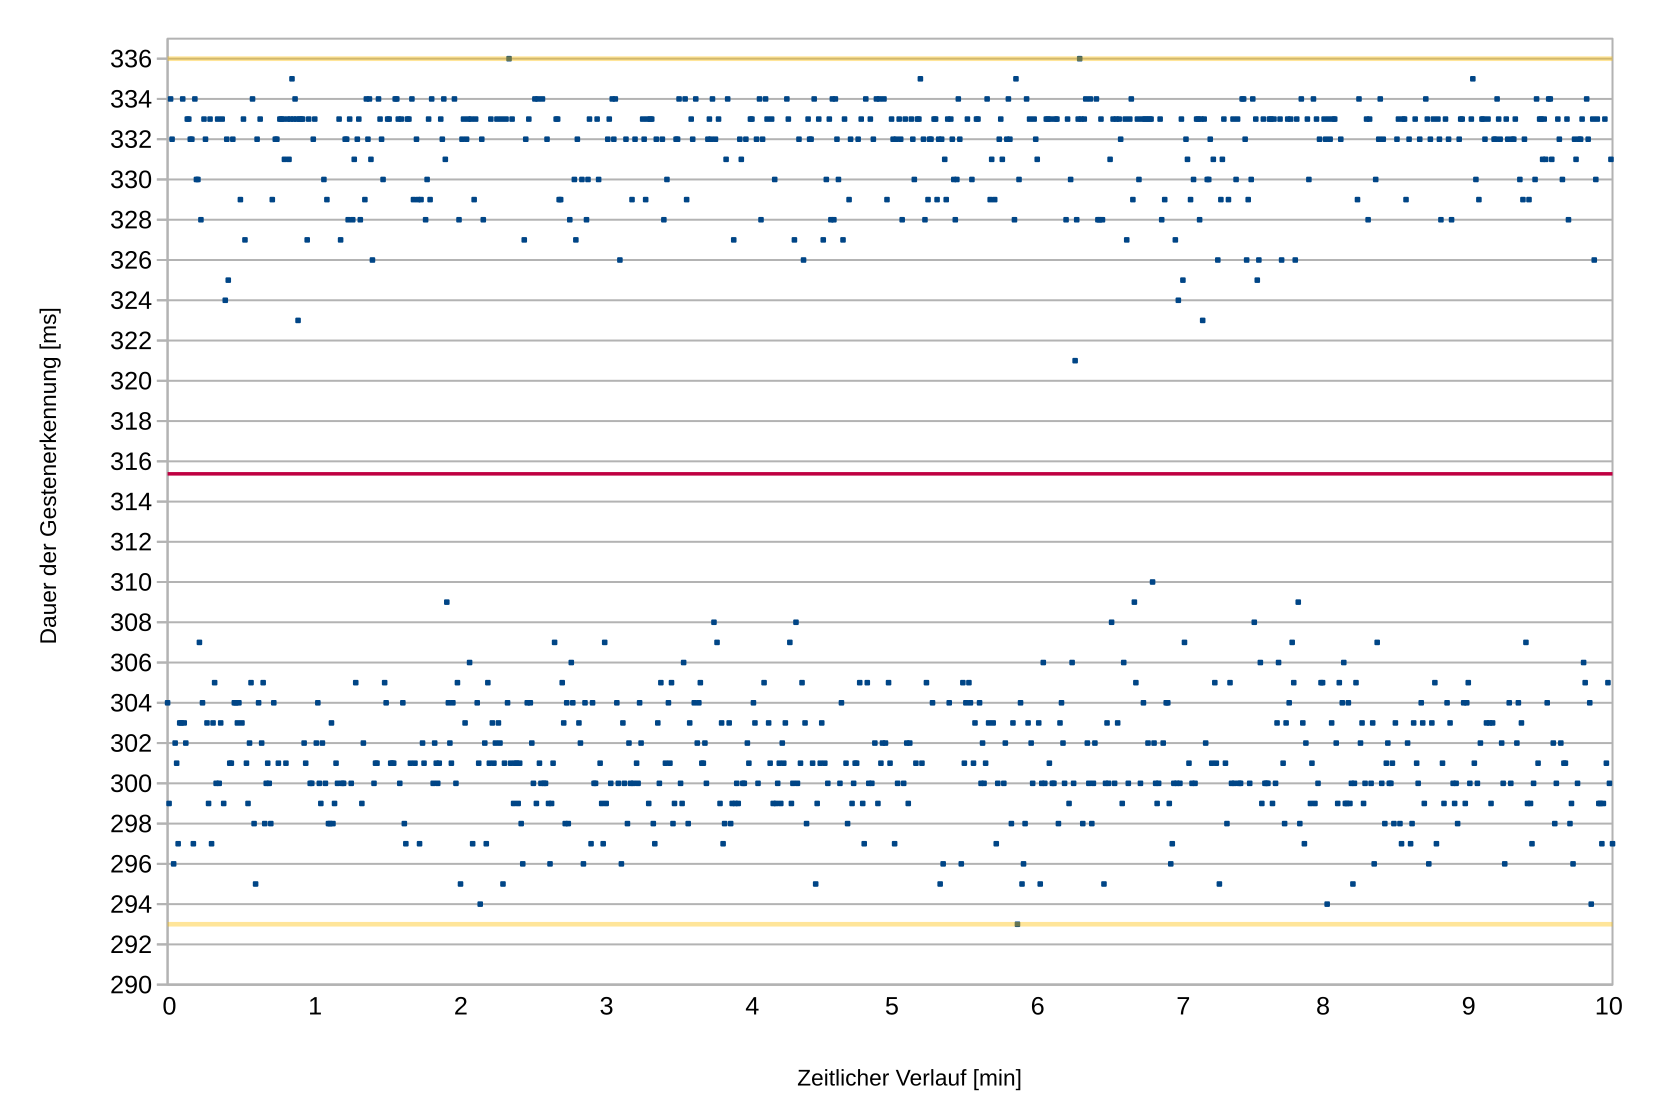
\includegraphics[width=1.04\textwidth]{images/ergebnisse/dauer_der_gestenerkennung_verlauf}
	\caption[Zeitlicher Latenzverlauf der Gestenerkennung der Azure Kinect]{Zeitlicher Latenzverlauf der Gestenerkennung der Azure Kinect\\Quelle: Eigene Ausarbeitung}
	\label{fig:measurement_gesture_recognition_azure_kinect}
\end{figure}
\FloatBarrier

In Abbildung \ref{fig:measurement_gesture_recognition_azure_kinect} ist zu sehen, dass der Mittelwert der Gestenerkennungsdauer, welcher durch die hellrote Linie visualisiert wird, in Richtung \num{326,29} ms tendiert. Die minimale Dauer der Gestenerkennung, welche durch die untere orange Linie visualisiert wird, beträgt \num{291} ms. Die maximale Dauer der Gestenerkennung, welche durch die obere orange Linie visualisiert wird, beträgt hingegen \num{366} ms. Die violette Linie stellt die Tendenz der Gestenerkennungsdauer dar, welche jedoch gleich zu bleiben scheint und hö́chstwahrscheínlich nur durch Schwankungen beeinflusst wird. Anzumerken ist, dass die Gestenerkennungsdauer sich im Durchschnitt stabil im Bereich zwischen \num{314,02} ms und \num{338,55} ms bewegt. Die annähernd gleich bleibende Gestenerkennungsdauer kann auf das DNN des Azure Kinect Body Tracking SDKs und den eingesetzten Prozess-Scheduler zurückgeführt werden. Eine nichtdeterministische Berechnung würde hierbei vermehrt Spikes und unvorhersagbarere Änderungen bei der Gestenerkennungsdauer bewirken. Nichtsdestotrotz liegen diese Werte weit über den 50 ms, welches für ein Teach Pendant empfohlen wird \cite[55]{prassler_advances_2004}. Zudem ist eine Verzögerung der Gestenerkennung bei über 100 ms für die bedienende Person bereits deutlich spürbar \cite{miller_response_1968}.

\section{Latenz der Roboter-Kommunikation mit und ohne ROS-Anbindung}
Zum Testen der Latenz der Roboter-Kommunikation mit und ohne ROS-Anbindung wurde bei der direkten Kommunikation zum Roboter die Latenz zwischen der aufrufenden Roboter-Gesten-Anwendung und der InterbotiX-Schnittstelle gemessen. Bei der ROS-Anbindung wird die Latenz der Kommunikation zwischen der Roboter-Gesten-Anwendung über den TCP/IP-Stack und daher über das Netzwerk bis hin zu der InterbotiX-Schnittstelle analysiert und gemessen. Bei der Untersuchung der Netzwerklatenz werden verschiedene praxisnahe Netzwerkkonstellationen simuliert um unvorhergesehene Netzwerklatenzen auffinden und diesen gegebenenfalls entgegenwirken zu können. Die Tests werden in einem Gigabit-Ethernet-Netzwerk durchgeführt, da Gigabit-Ethernet zum Zeitpunkt der Veröffentlichung dieser Arbeit als Standard angesehen wird und bereits weit verbreitet bei Routern und Clientsystemen ist \cite{gigabit_ethernet_2020}.\\

Zur Simulation der Netzwerkumgebungen wird NetEm mit Token Bucket Filter eingesetzt. NetEm stellt ein Netzwerkemulator dar und der Token Bucket Filter kann eine Warteschlange simulieren. Mithilfe von NetEm und Token Bucket Filter können verschiedene Netzwerkschnittstellen simuliert werden. Hierzu werden die im Linux-Kernel vorhandenen Möglichkeiten zur Steuerung des Netzwerkverkehrs eingesetzt. Bei ausgehenden Paketen können so Verzögerungen, Paketverlust, Duplizierung, Datenratenlimits und weitere Merkmale emuliert werden um eine Netzwerkschnittstelle an die Gegebenheiten eines vorhandenen Netzwerks anzupassen und z.B. Tests ohne die reale Netzwerkhardware reproduzierbar zu machen \cite{hemminger_network_nodate}. Ein Gigabit-Ethernet-Netzwerk, welches mit einem Router verbunden ist, kann wie in Listing \ref{lst:network_emulation_with_net_em} simuliert werden.\newline\vspace{-1.0em}

\begin{lstlisting}[style=bash, caption={Gigabit-Ethernet-Netzwerksimulation inklusive Simulation einer Routeranbindung mit NetEm und Token Bucket Filter}, label={lst:network_emulation_with_net_em}]
sudo tc qdisc add dev lo root handle 1: tbf rate 940Mbit burst 8192 limit 16384
sudo tc qdisc add dev lo parent 1:1 handle 10 netem corrupt 0.5% loss 0.1% delay \
0.2ms 0.05ms distribution normal reorder 3% 50%
\end{lstlisting}\leavevmode\newline\vspace{-1.0em}

In Listing \ref{lst:network_emulation_with_net_em} wird das Kommandozeilenprogramm \quoteMark{tc} verwendet um auf die Funktionalitäten von NetEm und des Token Bucket Filters zugreifen zu können. Zur Verwendung von \quoteMark{tc} werden Administratorrechte benötigt, da mit diesem Tool grundlegende Netzwerkeigenschaften, wie z.B. Datenraten, von vorhandenen Netzwerk-Interfaces, wie z.B. lo, eth*, eno* und wlo*, verändert werden können. \quoteMark{qdisc} ist die Abkürzung für \quoteMark{Queueing Discipline} und stellt den Netzwerkpakete-Scheduler von Linux dar, welcher die Netzwerkpakete entgegennimmt. Mit \quoteMark{add dev} kann ein Netzwerkinterface hinzugefügt werden um diesem bestimmte Netzwerkeigenschaften hinzufügen zu können. In diesem Fall wird \quoteMark{lo}, welches das Loopback-Interface darstellt und über \quoteMark{localhost} oder \quoteMark{127.0.0.1} angesprochen werden kann, ausgewählt. \quoteMark{root} und \quoteMark{parent} stellen hierbei Klassen dar, wobei einer \quoteMark{root}-Klasse eine \quoteMark{parent}-Klasse zugewiesen werden kann. Daher wird in Listing \ref{lst:network_emulation_with_net_em} über \quoteMark{parent 1:1} das erste verfügbare \quoteMark{root}-Element dem Netzwerk-Interface zugewiesen. Mit der Option \quoteMark{handle} wird ein Bezeichner zugewiesen über den die jeweilige Klasse angesprochen werden kann. Hierbei ist die Option \quoteMark{handle 1:} gleichbedeutend mit der Option \quoteMark{handle 1:0}. Aus diesem Grund kann daher über die Option \quoteMark{parent 1:1} auf die \quoteMark{root}-Klasse zugegriffen werden. Die Optionen \quoteMark{tbf} und \quoteMark{netem} spezifizieren den Toket Bucket Filter und NetEm. Mit \quoteMark{rate} kann zusätzlich die maximale Datenrate des Netzwerkinterface angegeben werden \cite{tc_net_em_nodate}. Bei einem Gigabit-Ethernet-Netzwerk kann hierbei eine Nettorate von 940 Mbit/s erreicht werden \cite{datendurchsatz_2020}. Die Option \quoteMark{burst} gibt an wie viele Bytes an Daten im Schnellzugriffs-Buffer gehalten werden können und die Option \quoteMark{limit} gibt an wie viele Bytes an Daten insgesamt in der Warteschlange gepuffert werden können bis diese gesendet werden müssen \cite{tc_net_em_nodate}. Bei Gigabit-Ethernet ist ein Burst von 8192 Bytes und ein Limit von 16384 Bytes möglich \cite{dembowski_lokale_2007}. Mit der Option \quoteMark{corrupt} kann die Anzahl fehlerhaften Pakete in Prozent angegeben werden. Die Option \quoteMark{loss} gibt an wie viele Pakete in Prozent über das Netzwerk verloren gehen sollen. Eine Verzögerung kann mit dem ersten Argument und eine Schwankung mit dem zweiten Argument von der Option \quoteMark{delay} spezifiziert werden. Eine Verteilungsfunktion kann dazu genutzt werden um eine der Verteilung ähnelnde Verzögerung zu erreichen. Die Pakete können zudem mit der Option \quoteMark{reorder} neu angeordnet werden um verspätete Netzwerkpakete zu simulieren. Das erste Argument der Option \quoteMark{reorder} gibt die Anzahl der neu anzuordnenden Pakete und das zweite Argument die Korrelation in Prozent an \cite{tbf_token_bucket_filter_nodate}. Bei Gigabit-Ethernet und einer Routeranbindung dazwischen ist eine Fehlerrate von \num{0,5}\%, eine Verlustrate von \num{0,1}\% und eine Verzögerung von \num{0,2} ms mit einer Schwankung von \num{0,05} ms und einer normalverteilten Verzögerung realitätsnah. Eine Neuanordnung der Netzwerkpakete von 3\% mit einer Korrelation von 50\% stellt eine praxisnahe Annäherung an die Gegebenheiten eines Gigabit-Ethernet-Netzerks mit Routeranbindung dar \cite{admin_understanding_2018}.\\

Bei der Durchführung der Tests wurden von dem Proband die in dieser Arbeit entwickelten Gesten abwechselnd in praxisnaher Reihenfolge vor der Azure Kinect ausgeführt um die Latenz der Kommunikation an einem praxisnahen Testbeispiel zu testen. Die Tests wurden zuerst an dem Loopback-Interface mithilfe des Gelenk-Modus ohne den in Listing \ref{lst:network_emulation_with_net_em} angegeben Beschränkungen getestet um eine lokale Interprozesskommunikation mithilfe des TCP/IP-Stacks zu testen. Anschließend wurden die in Listing \ref{lst:network_emulation_with_net_em} angegebenen Beschränkungen an drei verschiedenen Netzwerkkonstellationen angewandt und vom Proband im Weltkoordinatensystem- und Gelenk-Modus getestet. Die Netzwerkkonstellationen schließt hierbei eine Netzwerksimulation ohne zusätzlichen Netzwerktraffic und eine Netzwerksimulation mit hohem Netzwerktraffic mit ein um die zwei Randfälle testen zu können. Bei der Netzwerksimulation mit hohem Netzwerktraffic werden drei 4K-Bilder-ROS-Nodes simuliert um das Gigabit-Ethernet-Netzwerk mit einer Datenrate 1176 MB/s an seine maximale Grenze und darüber hinaus zu bringen. Dies stellt sicher, dass das Testnetzwerk zu jederzeit voll ausgelastet ist. Zum Testen der Latenz der Roboter-Kommunikation mit und ohne ROS-Anbindung wurde die Roboter-Gesten-Anwendung und deren Abhängigkeiten zudem mittels der Flags \quoteMark{MEASUREMENT} und \quoteMark{COMMUNICATION\_MEASUREMENT}, welche im Anhang \ref{appendix1.2:Installation_und_Konfiguration_der_Pakete} aufgezeigt werden, kompiliert. Die Dateien \quoteMark{interbotix\_robot\_arm\_communication\_measurement.csv} und \quoteMark{interbotix\_sdk\_communication\_measurement.csv}, welche von der Roboter-Gesten-Anwendung während der jeweiligen Tests erstellt wurden, sind in den jeweiligen Unterordnern \quoteMark{Messung der direkten Kommunikation}, \quoteMark{Messung der ROS-Kommunikation (ohne Netzwerksimulation)}, \quoteMark{Messung der ROS-Kommunikation (mit Netzwerksimulation \& niedriger Netzwerkauslastung)} und \quoteMark{Messung der ROS-Kommunikation (mit Netzwerksimulation \& hoher Netzwerkauslastung)} auf dem Beilagemedium im Verzeichnis \quoteMark{Testdaten/Messung der Kommunikation/} zu finden.

\begin{figure}[htb]
	\centering
	\includegraphics[width=1.04\textwidth]{images/ergebnisse/Messung_der_direkten_Kommunikation}
	\caption[Zeitlicher Latenzverlauf der direkten Kommunikation des \quoteMark{WidowX 200}-Lernroboters]{Zeitlicher Latenzverlauf der direkten Kommunikation des \quoteMark{WidowX 200}-Lernroboters\\Quelle: Eigene Ausarbeitung}
	\label{fig:measurement_robot_direct_communication}
\end{figure}
\FloatBarrier

Bei der Messung der direkten Kommunikation zum \quoteMark{WidowX 200}-Lernroboter, welche in Abbildung \ref{fig:measurement_robot_direct_communication} ersichtlich ist, konnte eine nicht messbare Verzögerung von deutlich unter 1 ms festgestellt werden. Dies ist damit zu erklären, weil die Kommunikation zwischen der Roboter-Gesten-Anwendung über einen geteilten Speicherbereich erfolgt und die Übertragung der Steuerungsbytes zum \quoteMark{WidowX 200}-Lernroboter über das \quoteMark{USB 2.0}-Kabel aufgrund der geringen Datenmenge mit einer nicht messbaren Verzögerung erfolgen kann. Zudem kann davon ausgegangen werden, dass die Kommunikation der Roboter-Gesten-Anwendung mit der InterbotiX-Schnittstelle sehr effizient erfolgt. Die in Abbildung \ref{fig:measurement_robot_direct_communication} z.T. ersichtlichen schmalen Spalte zwischen den grünen Punkten enstanden durch das Außsetzen oder durch das Nichterkennen der vom Proband durchgeführten Gestenbewegungen. Aufgrund der geringen Kommunikationslatenz zwischen der Roboter-Gesten-Anwendung und der InterbotiX-Schnittstelle ist daher die direkte Kommunikation mit dem \quoteMark{WidowX 200}-Lernroboter wegen der kurzen Übertragungsdauer vernachlässigbar klein. Bei den Tests mit der Netzwerkkommunikation kann daher davon ausgegangen werden, dass die Netzwerkkommunikation einen signifikanteren Einfluss auf die Kommunikationslatenz als die Übertragung der Steuerungsbytes zum \quoteMark{WidowX 200}-Lernroboter über das \quoteMark{USB 2.0}-Kabel haben wird.

\begin{figure}[htb]
	\centering
	\includegraphics[width=1.04\textwidth]{images/ergebnisse/Messung_der_ROS_Kommunikation_App_und_keine_Netzwerksimulation}
	\caption[Zeitlicher Latenzverlauf der ROS-Kommunikation des \quoteMark{WidowX 200}-Lernroboters (ohne Netzwerksimulation)]{Zeitlicher Latenzverlauf der ROS-Kommunikation des \quoteMark{WidowX 200}-Lernroboters (ohne Netzwerksimulation)\\Quelle: Eigene Ausarbeitung}
	\label{fig:measurement_robot_ros_without_network_simulation}
\end{figure}
\FloatBarrier

Bei der Messung der ROS-Kommunikation über das Loopback-Interface und ohne eine Netzwerksimulation konnte ein Anstieg von Durchschnittlich 30 ms im Gegensatz zur direkten Kommunikation verzeichnet werden. Dies ist damit zu erklären, dass die Kommunikation über den TCP/IP-Stack erfolgt und daher der Netzwerk-Overhead mit zu berücksichtigen ist. Die minimale Latenzzeit der ROS-Kommunikation über das Loopback-Interface, welche durch die untere orange Linie visualisiert wird, beträgt im Extremfall \num{12} ms. Die maximale Latenzzeit der ROS-Kommunikation über das Loopback-Interface, welche durch die obere orange Linie visualisiert wird, beträgt hingegen im Extremfall \num{57} ms. Die Latenzzeit liegt im Durchschnitt zwischen 23 ms und 36 ms. Es ist zudem zu erwähnen, dass der Proband am Anfang des Tests für 30 Sekunden im Weltkoordinatensystem-Modus, danach bis 6 Minuten nach dem Start des Tests im Gelenk-Modus und anschließend wieder im Weltkoordinatensystem-Modus die praxisnahen Gestenbewegungen durchgeführt hatte. Dies zeichnet sich auch durch die violette Linie aus, welche die Tendenz der Latenzzeit widerspiegelt. Anzumerken ist zudem, dass beim Weltkoordinatensystem-Modus zuerst ein Plan erstellt werden muss und dieser daraufhin über das Netzwerk und daher über den TCP/IP-Stack zur Roboter-Gesten-Anwendung übertragen werden muss. Daraufhin kann der erzeugte Plan von der Roboter-Gesten-Anwendung über das Netzwerk und daher über den TCP/IP-Stack von MoveIt an den InterbotiX-Node weitergeleitet werden. Aufgrund der extremen Schwankungen ist es womöglich empfehlenswert zeitkritische Steuerungsbefehle mehrmals zu senden um sicherzugehen, dass diese auch zeitgerecht ankommen. Hierzu müsste jedoch ein Algorithmus implementiert werden um identische Steuerungsbefehle erkennen und ein mehrmaliges Ausführen der Steuerungsbefehle verhindern zu können.

\begin{figure}[htb]
	\centering
	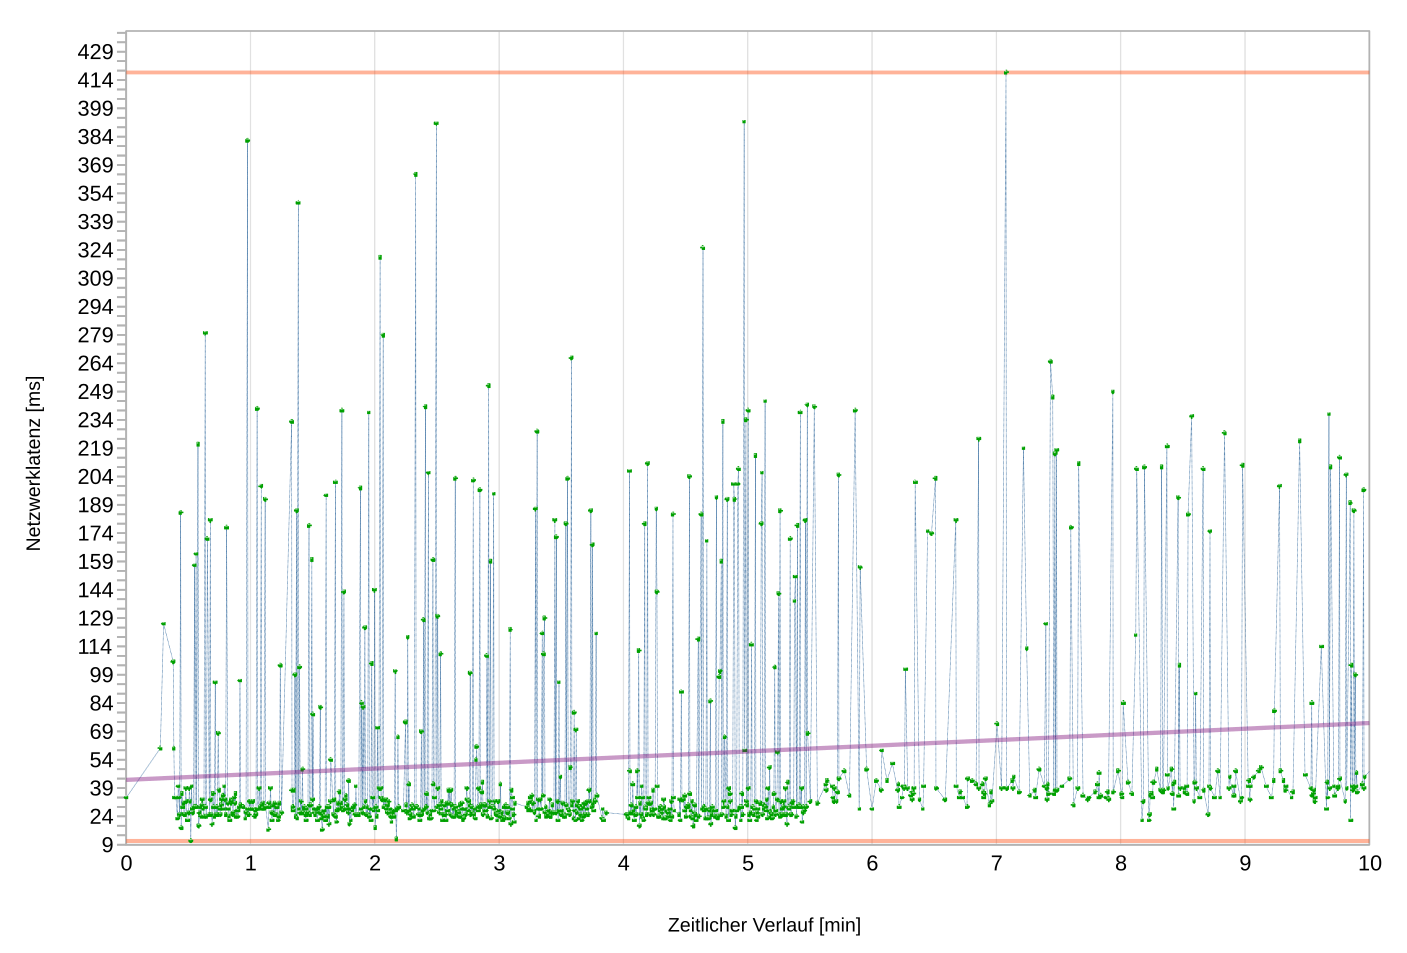
\includegraphics[width=1.04\textwidth]{images/ergebnisse/ROS_App_und_mit_Netzwerksimulation}
	\caption[Zeitlicher Latenzverlauf der ROS-Kommunikation des \quoteMark{WidowX 200}-Lernroboters (mit Netzwerksimulation \& niedriger Netzwerkauslastung)]{Zeitlicher Latenzverlauf der ROS-Kommunikation des \quoteMark{WidowX 200}-Lernroboters (mit Netzwerksimulation \& niedriger Netzwerkauslastung)\\Quelle: Eigene Ausarbeitung}
	\label{fig:measurement_robot_ros_with_network_simulation_low_network_traffic}
\end{figure}
\FloatBarrier

Bei der Messung der ROS-Kommunikation über das Gigabit-Ethernet-Netzwerk mit einer Netzwerksimulation und einer niedrigen Netzwerkauslastung stellte sich wie erwartet heraus, dass die Latenzeit bei der Kommunikation über das Gigabit-Ethernet-Netzwerk zu mehr Spikes als mit dem Loopback-Interface tendiert. Es ist wiederum anzumerken, dass der Proband am Anfang des Tests für 30 Sekunden im Weltkoordinatensystem-Modus, danach bis 5 Minuten und 30 Sekunden nach dem Start des Tests im Gelenk-Modus und anschließend wieder im Weltkoordinatensystem-Modus die praxisnahen Gestenbewegungen durchgeführt hatte. Dies zeichnet sich auch durch die violette Linie aus, welche die Tendenz der Latenzzeit widerspiegelt. Bei der Messung der ROS-Kommunikation über das Gigabit-Ethernet-Netzwerk und ohne eine Netzwerksimulation konnte ein Anstieg von mindestens 20 ms im Gegensatz zur ROS-Kommunikation ohne Netzwerksimulation verzeichnet werden. Die minimale Latenzzeit der ROS-Kommunikation über das Gigabit-Ethernet-Netzwerk, welche durch die untere orange Linie visualisiert wird, beträgt im Extremfall \num{11} ms. Die maximale Dauer der Gestenerkennung, welche durch die obere orange Linie visualisiert wird, beträgt hingegen im Extremfall \num{418} ms. Die Latenzzeit liegt im Durchschnitt jedoch zwischen 18 ms und 116 ms. Dies ist damit zu erklären, dass die Kommunikation über ein realitätsnahes Netzwerk erfolgt und daher der Netzwerk-Overhead und der Overhead des Routers mit zu berücksichtigen ist. Aufgrund der Spikes von Durchschnittlich bis zu 116 ms ist es zudem unmöglich die 50 ms, welches für ein Teach Pendant empfohlen werden \cite[55]{prassler_advances_2004}, einzuhalten.

\begin{figure}[htb]
	\centering
	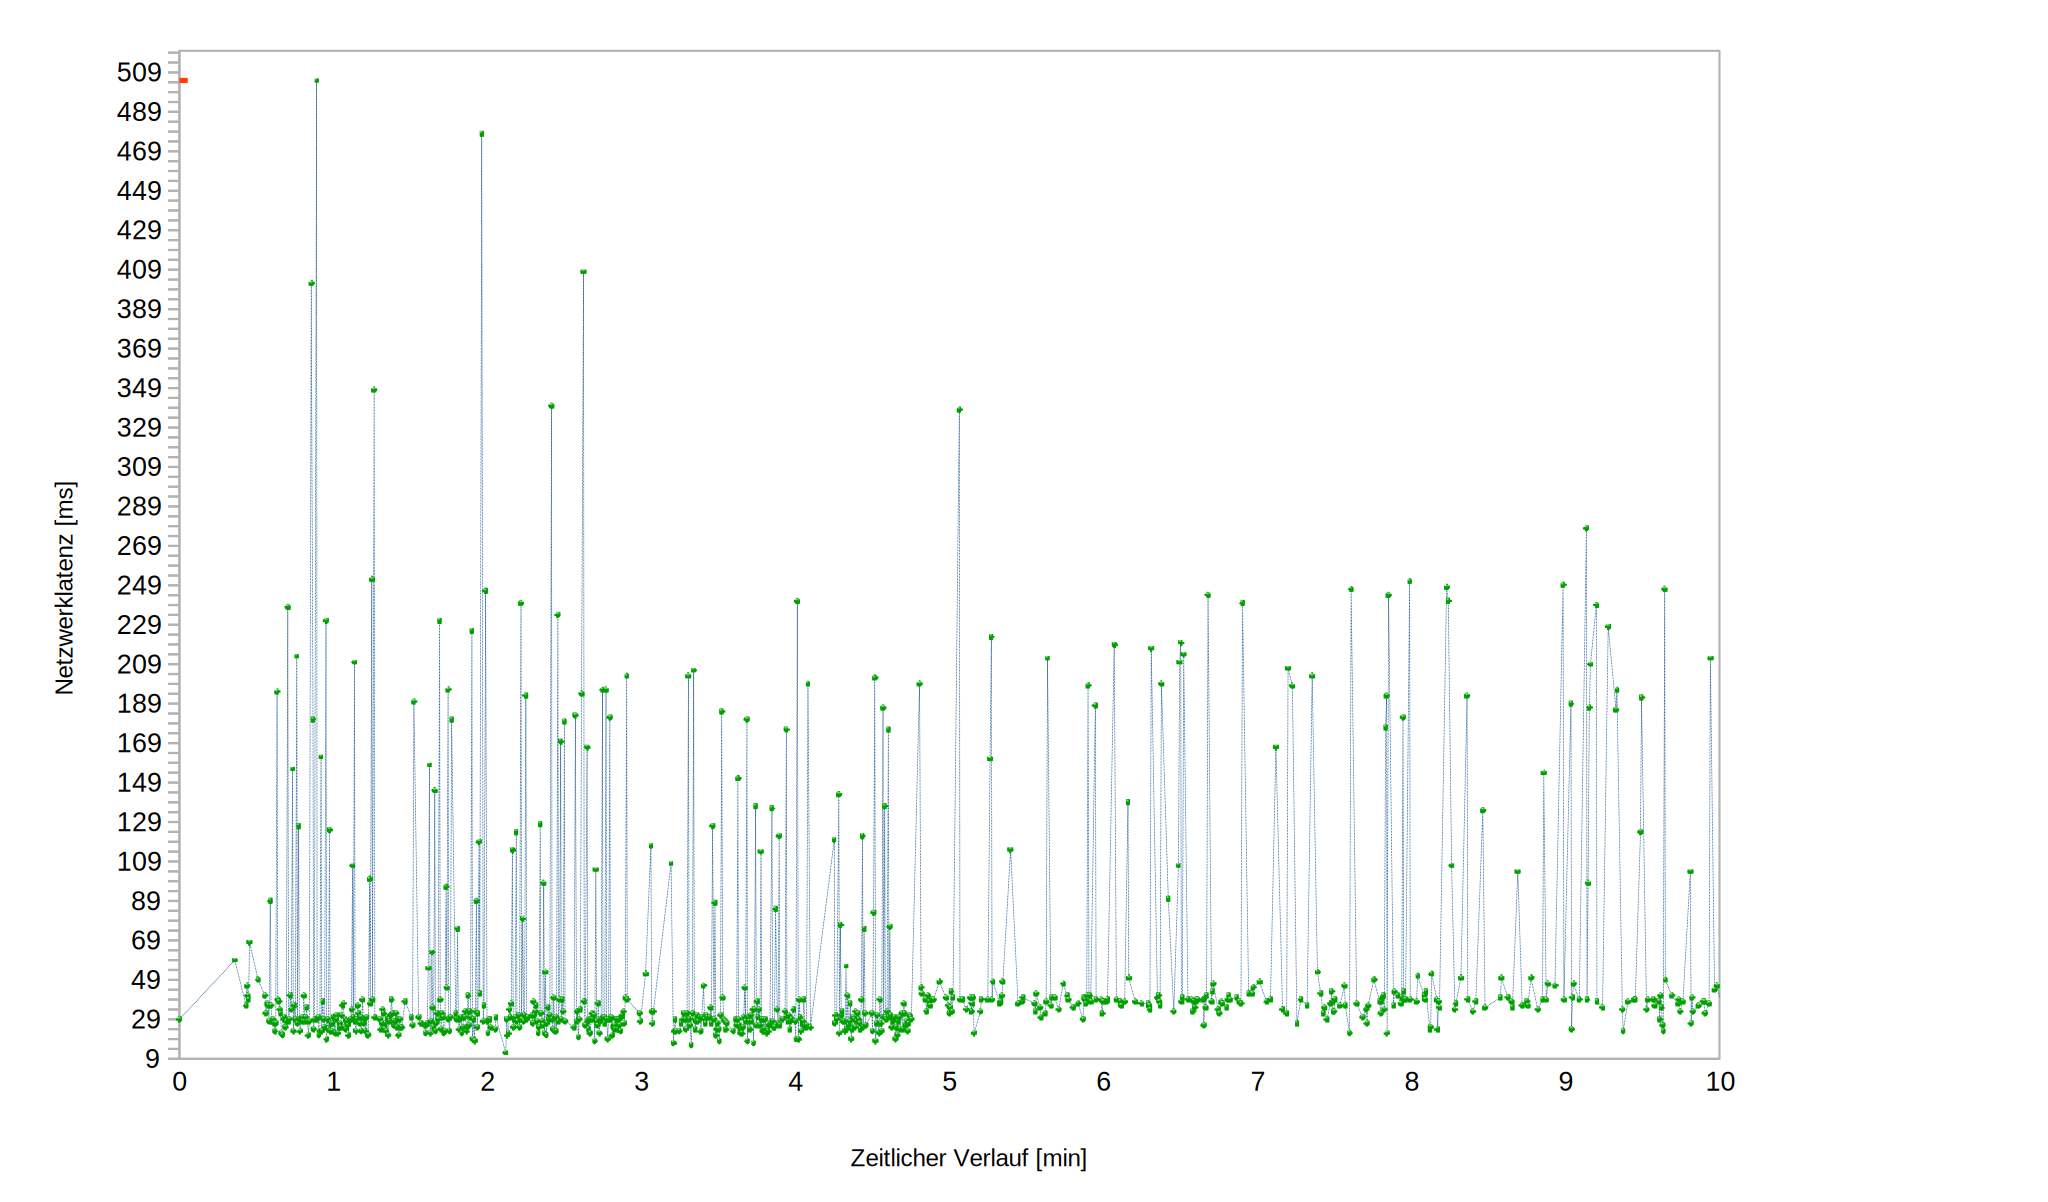
\includegraphics[width=1.04\textwidth]{images/ergebnisse/ROS_App_mit_Netzwerksimulation_und_hohe_Auslastung}
	\caption[Zeitlicher Latenzverlauf der ROS-Kommunikation des \quoteMark{WidowX 200}-Lernroboters (mit Netzwerksimulation \& hoher Netzwerkauslastung)]{Zeitlicher Latenzverlauf der ROS-Kommunikation des \quoteMark{WidowX 200}-Lernroboters (mit Netzwerksimulation \& hoher Netzwerkauslastung)\\Quelle: Eigene Ausarbeitung}
	\label{fig:measurement_robot_ros_with_network_simulation_high_network_traffic}
\end{figure}
\FloatBarrier

Bei der Messung der ROS-Kommunikation über das Gigabit-Ethernet-Netzwerk mit einer Netzwerksimulation und einer hohen Netzwerkauslastung stellte sich heraus, dass die Latenzeit bei der Kommunikation über das Gigabit-Ethernet-Netzwerk dazu tendiert annähernd gleich zu bleiben. Es konnte zudem kein signifikanter Anstieg im Gegensatz zur ROS-Kommunikation mit Netzwerksimulation und geringer Netzwerkauslastung verzeichnet werden. Nur die maximale Latenzzeit stieg auf 505 ms an, was jedoch aufgrund der geringen Häufigkeit als Ausreißer anzusehen ist. Es ist zudem zu erwähnen, dass der Proband am Anfang des Tests für 30 Sekunden im Weltkoordinatensystem-Modus, danach bis 5 Minuten nach dem Start des Tests im Gelenk-Modus und anschließend wieder im Weltkoordinatensystem-Modus die praxisnahen Gestenbewegungen durchgeführt hatte. Da bei den Tests mit niedriger und hoher Netzwerkauslastung annähernd die gleichen Latenzeiten gemessen wurden, lässt darauf schließen, dass die zu Übertragende geringe Datenmenge der Steuerungsbefehle und der Planungsdaten die Ursache hierfür darstellt. Bei größeren zu übertragenden Datenmengen wäre das Ergebnis höchstwahrscheinlich unterschiedlicher ausgefallen. Nichtsdestotrotz konnte ermittelt werden wie ROS in überschaubaren Anwendungen mit hoher Netzwerkauslastung zurechtkommt.

\section{Genauigkeit der Zielpositionen}
Zum Testen der Genauigkeit der Zielpositionen wurde wiederum das das Azure Kinect Body Tracking SDK im CPU-Modus anstatt mit der Grafikkartenbeschleunigung gestartet. Zudem stand es dem Proband, welcher bereits sehr efahren mit der Roboter-Gesten-Anwendung ist, frei zwischen dem Weltkoordinatensystem- und Gelenk-Modus zu wechseln um die anzufahrenden Zielpositionen, wie in Abbildung \ref{fig:white_page_with_folded_corner} zu sehen sind, anzusteuern. Ziel war es mit den Mittelpunkt des TCPs so exakt wie nur möglich über dem Mittelpunkt der roten Kreuzes zu platzieren. Die Zeitdauer wurde zudem erfasst um auswerten zu können ob die benötigte Zeitdauer einen Einfluss auf die Genauigkeit der anzufahrenden Zielpositionen hatte. Um die Messung der angefahrenen Zielpositionen genauer durchführen und analysieren zu können, wurde der Test im Simulator Gazebo durchgeführt. In der Simulationsumgebung wurde hierfür ein virtueller Raum erschaffen, in welchem die exakten Zielpositionen bereits genau vordefiniert sind. Die ermittelten Positionen konnten daraufhin mit den exakten Positionen verglichen und die Differenzen ermittelt werden. Für diesen Testfall wurde die Roboter-Gesten-Anwendung und deren Abhängigkeiten mittels der Flags \quoteMark{MEASUREMENT} und \quoteMark{POSITION\_MEASUREMENT}, welche im Anhang \ref{appendix1.2:Installation_und_Konfiguration_der_Pakete} aufgezeigt werden, kompiliert. Die Dateien \quoteMark{position\_measurement.csv}, \quoteMark{robot\_arm\_positions.json}, \quoteMark{gazebo\_state.log},  \quoteMark{Gazebo.mp4} und \quoteMark{Durchführung der Gesten.mp4}, welche bei der Durchführung des Tests erstellt wurden, sind auf dem Beilagemedium im Verzeichnis \quoteMark{Testdaten/Messung der Zielpositionen/} zu finden.

\begin{figure}[htb]
	\centering
	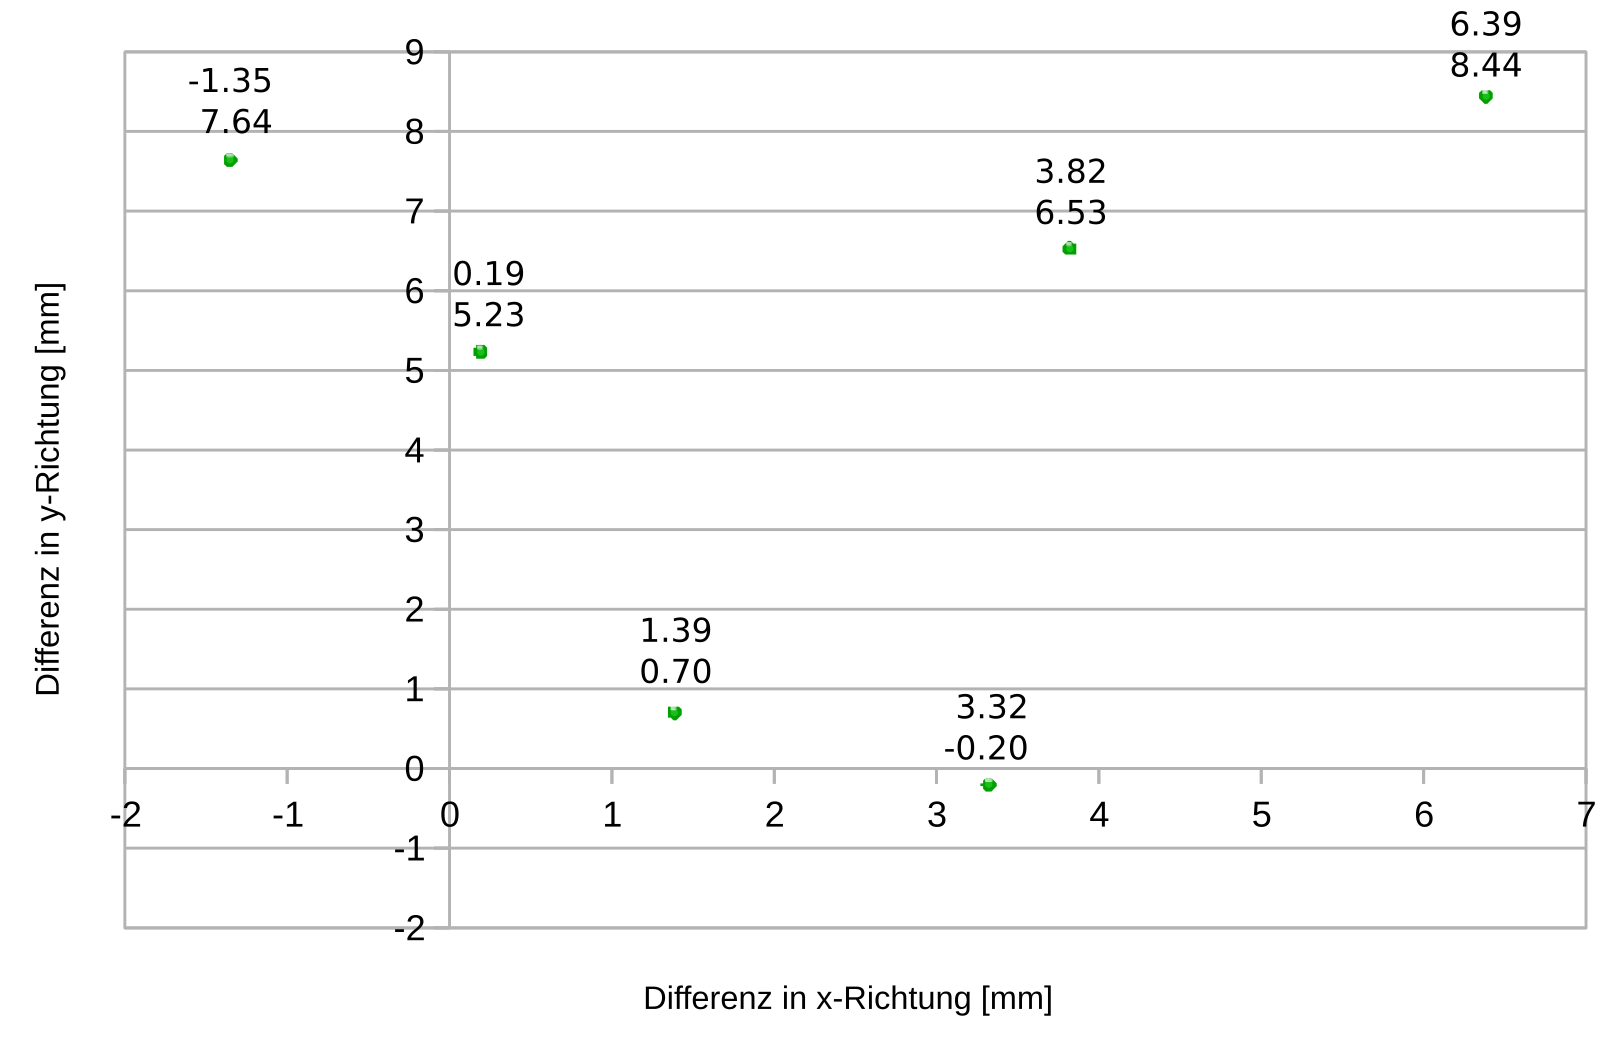
\includegraphics[width=0.808\textwidth]{images/ergebnisse/Differenzen_beim_Teachen_mit_Gesten}
	\caption[Positionsdifferenzen beim Teachen mit der Roboter-Gesten-Anwendung]{Positionsdifferenzen beim Teachen mit der Roboter-Gesten-Anwendung\\Quelle: Eigene Ausarbeitung}
	\label{fig:measurement_teaching_positions_differences}
\end{figure}
\FloatBarrier

In Abbildung \ref {fig:measurement_teaching_positions_differences} sind die Differenzen in x- und y-Richtung zu den sechs angefahrenen Zielpositionen eingetragen. Es ist zu sehen, dass maximal eine Differenz in von \num{8,44} mm und minimal eine Differenz von \num{0,20} mm in eine Richtung erreicht wurden. Die Differenz in x- und y-Richtung ist ansonsten jedoch annähernd gleich und der Unterschied kann als vernachlässigbar klein angesehen werden. Die erzielten Differenzen liegen im zuvor angenommenen Bereich von wenigen Millimetern und sind daher für den \quoteMark{WidowX 200}-Lernroboter akzeptabel. Für einen Industrieroboter wären hierbei höhere Genauigkeiten wünschensert. Da jedoch die Zielpositionen im Nachhinein angepasst werden können ist dieser Mangel jedoch unwesentlich klein.

\begin{figure}[htb]
	\centering
	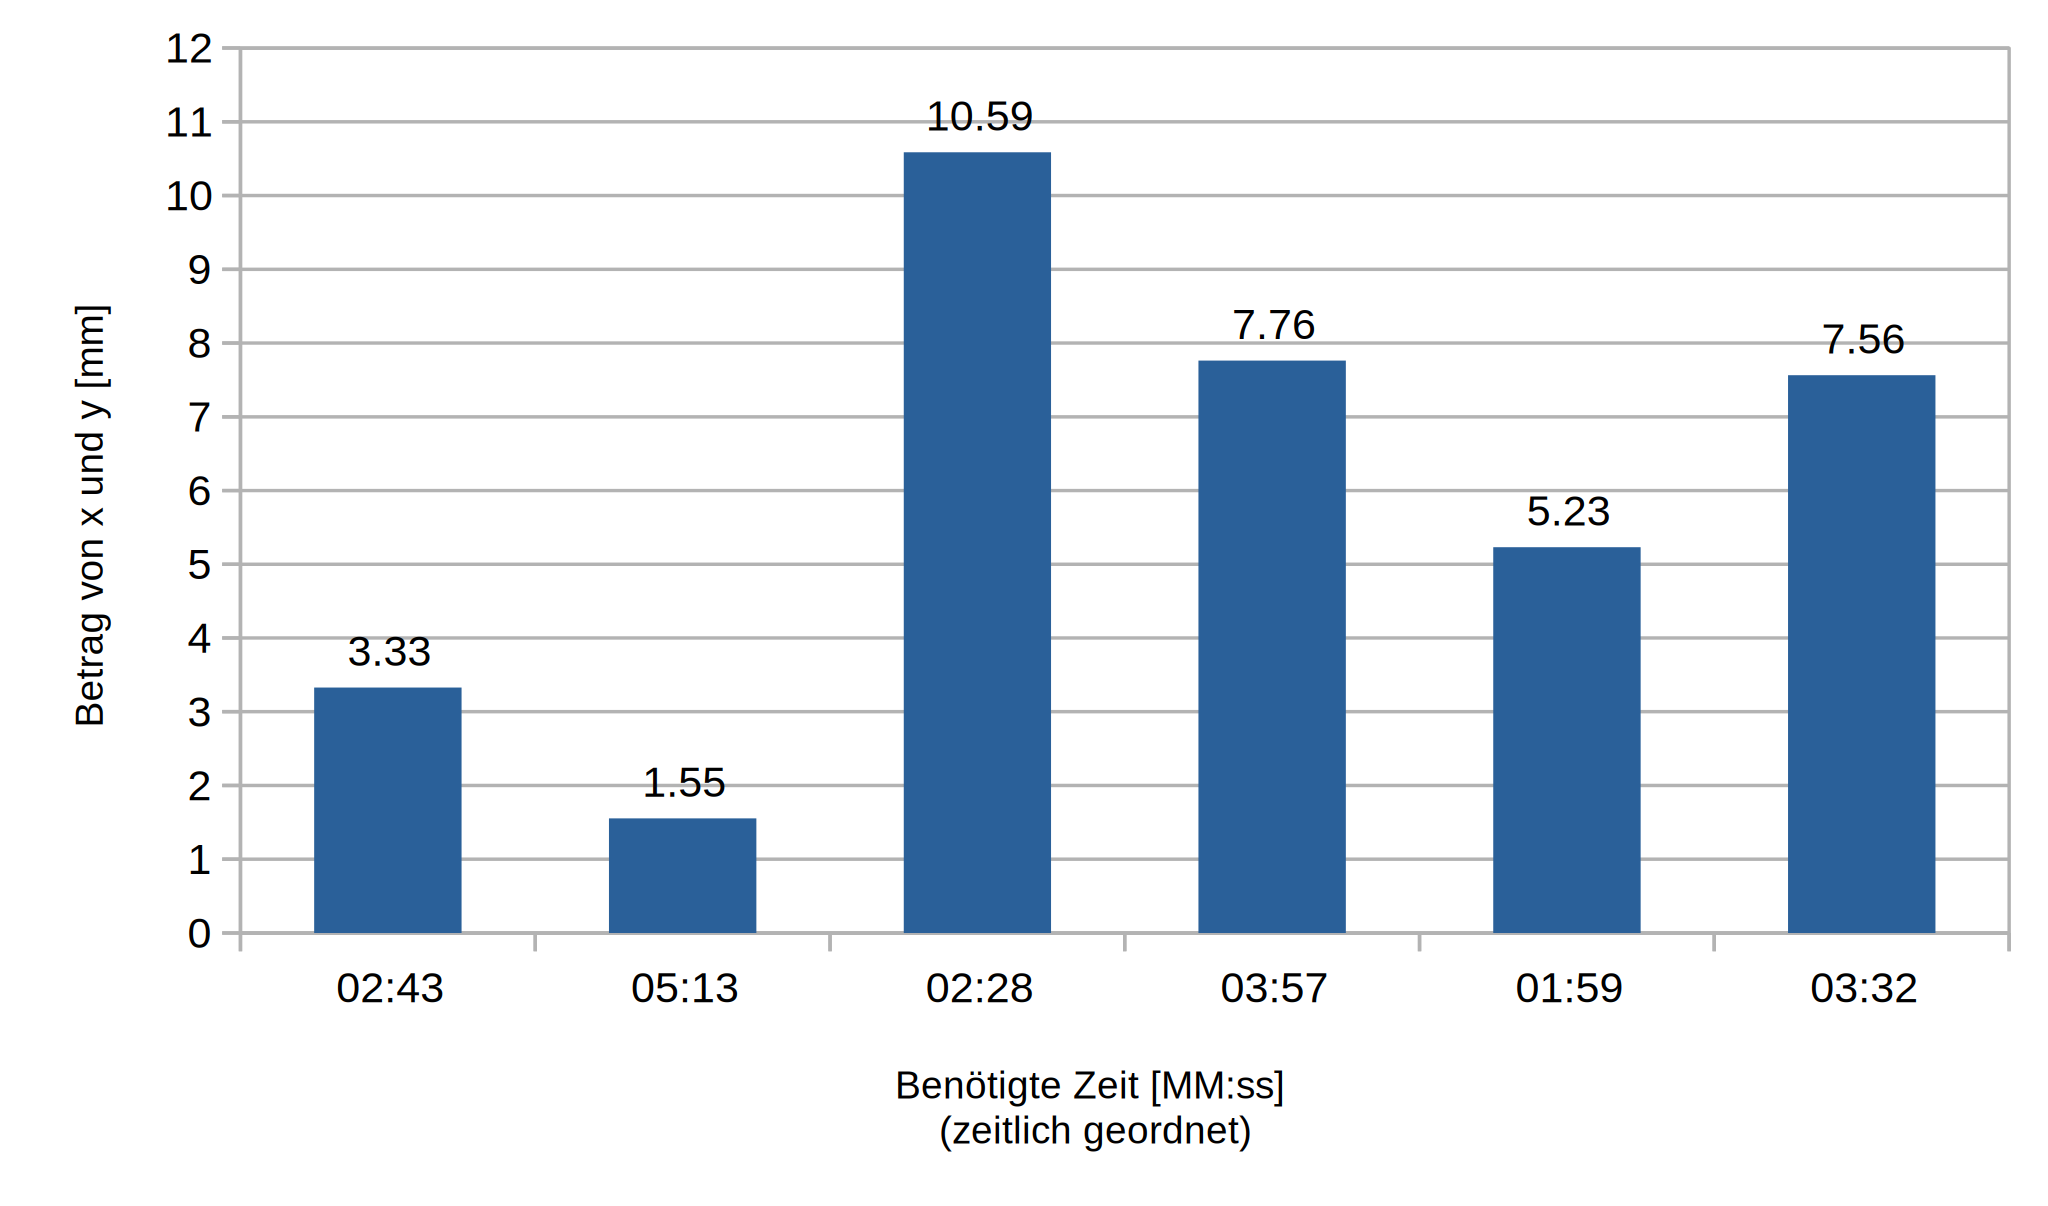
\includegraphics[width=0.808\textwidth]{images/ergebnisse/Betrag_der_Fehlerquadrate}
	\caption[Betrag der Fehlerquadrate beim Teachen mit der Roboter-Gesten-Anwendung]{Betrag der Fehlerquadrate beim Teachen mit der Roboter-Gesten-Anwendung\\Quelle: Eigene Ausarbeitung}
	\label{fig:measurement_teaching_positions_time_and_errors}
\end{figure}
\FloatBarrier

Bei Betrachtung der benötigten Zeit und der dazugehörigen Genauigkeit für diesen Test, wie in Abbildung \ref{fig:measurement_teaching_positions_time_and_errors} zu sehen ist, kann gesagt werden bei zunehmender Teach-Dauer des \quoteMark{WidowX 200}-Lernroboters auch die Genauigkeit abgenommen hat. Dabei wurden die ersten zwei Zielpositionen noch mit der geringsten Fehlerrate angefahren. Ab der dritten Zielposition war die größte Differenz. Danach hat sich die Differenz jedoch normalisiert und auf eine fast gleich bleibenden Fehlerrate gesenkt. In den meisten Fällen in denen die benötigte Zeit zum Anfahren einer Zielposition länger gewählt wurde, verringerte sich auch zumeist die Fehlerrate. Die durchschnittliche Teachdauer zum Erreichen der Zielpositionen lag in diesen Testbeispielen bei ca. 3 Minuten. Abschließend kann gesagt werden, dass die Fehlerrate bei sechs anzufahrenden Zielpositionen im tolerierbaren Wertebereich bleibt und bei längerer Benutzung der Roboter-Gesten-Anwendung annähernd gleichbleibend ist.

\section{Genauigkeit der Gestenerkennung}
Bei Analyse der Aufnahme \quoteMark{Durchführung der Gesten.mp4}, welches auf dem Beilagemedium im Verzeichnis \quoteMark{Testdaten/Messung der Zielpositionen/} zu finden ist, stellte sich heraus, dass der Proband mehrmals reflexartige Bewegungen durchgeführt und die Brille zudem am Brillensteg hinaufgeschoben hatte. Reflexartige Bewegungen gehen zumeist unterbewusst vonstatten, wie auch das hinaufschieben der Brille, welches zumeist aus Bequenlichkeitsgründen unterbewusst durchgeführt wird \cite{matschnig_glossar_nodate}. Es kann aufgrund der Aufnahme gesagt werden, dass die Roboter-Gesten-Anwendung zumindest gegen die genannten reflexartige und unterbewusste Bewegungen gesichert ist.
